\chapter{Experiments, Results and Analysis}\label{chap:experiments_and_results}

% Present the chapter
In this Chapter the experiment design is presented. Results are shown and an in
depth analysis is conducted, including: Energy and distance metrics for
measuring the performance of the proposed methods; A rigorous statistic testing
of the proposed methods; A comparison to competing methods in the literature in
order to validate the proposed methods; Finally, a visual inspection of the
best predictions and a comparison against the native conformation.
\textcolor{red}{TODO: tem q atualizar aqui conforme for escrevendo}

\section{Design of Experiments}\label{sec:design_of_experiments}

% Present the hardware setup
The experiments were all conducted on a single machine using the same hardware
throughout the full experimentation. Table~\ref{tab:machine-setup}
presents the machine utilized to run all the experiments. Each run of a
prediction method consists of a serial program that run continually without
interruption. The experiments were run in parallel, limited to at most one
running test per core\footnote{Only physical cores were considered. No virtual
(Hyperthreading) core was involved in the computations.}. To ensure maximum
repeatability the machine had no graphical interface enabled or any other form
of user interaction during the course of the experimentation.

\begin{table}[th]
    \centering
    \begin{tabular}{r|l} \hline \hline
        Name & Value \\ \hline \hline
        Operating System & Arch Linux \\ \hline
        Kernel &  Arch Linux Kernel 4.18.16 \\ \hline
        CPU & Intel(R) Core(TM) i5-3570K CPU @ 4.20GHz \\ \hline
        Number of Cores & 4 Physical cores, no hyperthreading cores \\ \hline
        RAM & 16 GB @ 1400 MHz \\ \hline \hline
    \end{tabular}
    \caption{The Machine Setup}
    \label{tab:machine-setup}
\end{table}

The experimentation consisted of running the two proposed methods, namely
SADE-REMC-FINAL and SADE-MC-FINAL. Two of the methods proposed
in~\cite{silva2019self} are also included, Namely SADE-REMC and SADE-MC.
Lastly, the Rosetta Ab Initio protocol is also included, amounting to five
different methods being ran.

The analysis is divided in two steps. In the first one, the two proposed methods
are compared agaisnt the works in~\cite{silva2019self} and the Rosetta Ab Initio
Protocol.
% Present the "in house" comparison
The metrics utilized in this are the \textit{scorefxn} energy value of the
best solution and the \ac{RMSD} associated with the same conformation. The
results were collected over 50 independent runs of each method for each target
protein. A graphical analysis is conducted in order to identify visually the
relative performance between the proposed methods. Considering that a visual
analysis is not enough (in this case), a more rigorous numerical statistic set
of test is conducted.  The Shapiro-Wilk~\cite{wilk1968joint} normality test is
employed with a confidence level of 5\%, i.e. $\alpha = 0.05$, to assess the
presence (or lack) of a underlying normal distribution. Based on its result, a
parametric/non-parametric test is employed with a confidence level of $\alpha =
0.05$. Due to the multiple comparisons involved \v{S}idák's $\alpha$ correction
will be utilized~\cite{vsidak1967rectangular}. The winner (or winners)
method(s) will be used in further comparison against the literature. The
processing time for this stage is also analyzed. The time required from the
start of the initial population generation until the final full atom model
output is measured in seconds.
\textcolor{red}{TODO: colocar parameter control analysis}
\textcolor{red}{TODO: convergence analysis}
\textcolor{red}{TODO: ffi analysis}
\textcolor{red}{TODO: mc vs remc analysis}

% Explain the clustering results
The use of clustering to extract and return different conformations from the
proposed methods require extra steps during the analysis. First, the main use of
returning several conformations is to allow an human expert to choose one that
has the desired properties. This, can not be automated in a test enviroment where
hundres of experiments are performed computationaly each day. As such, the human
expert, for the purposes of performance evaluation, must be replaced by a
computer oracle. This oracle can always find the conformation with the lowest
RMSD or the conformation with the lowest energy. This, of course, would not
be possible in a real world scenario where a protein without a know structure is
being predicted. With that in mind, the analysis of the two proposed methods is
devided in two sub groups. The first is named \texttt{best-by-rmsd} and the second
is named \texttt{best-by-energy}.

% Present the "free for all" analysis
In the second analysis step, a direct comparison against several works in the
literature is considered. Since there is a severe lack of standardization in the
literature regarding experimentation, the following methodology was used. Works
that provided the best RMSD had their proteins listed. The proteins that occured
the most were used for comparison. It is worth noting that the majority of works
provide little information about how the experimentation was conducted. The way
in which the results are analysed lacks a standard. As such, this work does a
direct comparison using the best RMSD achieved in a set of runs. While this is
not ideal, due to different works running each method different number of times,
this is possibly the only way to a comparison against several works. The presence
of outliers also weaken this comparison. Also, since only the most used proteins
are select, it is possible that some works are only represented partially, i.e.
some of the results are left out. Nevertheless, at the end of the day for the
PSPP what matters is having the lowest possible error. As such, comparing just
the best RMSD still a worthwhile analysis, albeit not ideal.

% Present the protein set
With that in mind, the set of proteins presented in Table~\ref{tab:protein-targets}
was chosen. The column \textbf{Name} contains the protein identification code
as in PDB.  The \textbf{Size} column shows the number of amino acids in the protein.
The \textbf{Backbone Angles} column shows the number of angles in the backbone,
this also has a one to one relation to the number of variables to be optimized
for a given protein. The \textbf{Structure} column holds the secondary
structures present in the protein set represented by $\alpha$-helices or
$\beta$-sheets.

\begin{table}[bh]
  \centering
  \begin{tabular}{ l | c | c | c | c }
    \hline \hline
    Name & Size & Backbone Angles & Structure         \\ \hline \hline
    1L2Y & 20   & 60              & $2\alpha$         \\ \hline
    1WQC & 26   & 78              & $2\alpha$         \\ \hline
    1ACW & 29   & 87              & $1\alpha, 2\beta$ \\ \hline
    1ZDD & 35   & 105             & $2\alpha$         \\ \hline
    2MR9 & 44   & 132             & $3\alpha$         \\ \hline
    1CRN & 46   & 138             & $2\alpha, 2\beta$ \\ \hline
    1ENH & 54   & 162             & $3\alpha$         \\ \hline
    1ROP & 63   & 189             & $2\alpha$         \\ \hline
    1UTG & 70   & 210             & $4\alpha$         \\ \hline
    1AIL & 72   & 216             & $3\alpha$         \\ \hline
    \hline
  \end{tabular}
  \caption{Target proteins and their features}
  \label{tab:protein-targets}
\end{table}

% present each protein (or maybe not)

% present the two algorithms (MC vs REMC)

% Present the parameters
The two proposed methods all operates with the same parameters, as presented
in~\ref{tab:parameters}.The first columns contains the parameter name and the
second one its respective value. The SaDE learning Phase has its default value,
as presented in~\cite{qin2009differential}. There are 100 simultaneous
trajectories throughout the execution, i.e. a population size of 100. A million
function evaluations are available for the optimization phase, where each
fragment insertion routine can use up to 25 at a time. \ac{FFI} uses a fragment
size of 9 and is applied with a probability of 2\% before each standard fragment
insertion. The other methods being compared uses the same values from
Table~\ref{tab:parameters} as apliable.

\begin{table}[ht]
    \centering
    \begin{tabular}{r|l} \hline \hline
        Parameter & Value \\ \hline \hline
        SaDE learning Phase & 50 \\ \hline
        Population Size & 100 \\ \hline
        Function Evaluation Budget & 1000000 \\ \hline
        MC/REMC Function Evaluation Budget & 25 \\ \hline
        Spicker cluster size & 10 \\ \hline
        Crowding factor & 5 \\ \hline
        Crowding distance method & RMSD \\ \hline
        \ac{FFI} probability & 0.02 \\ \hline
        \ac{FFI} length & 9 \\ \hline \hline
    \end{tabular}
    \caption{Parameters utilized in the proposed methods}
    \label{tab:parameters}
\end{table}

\section{Energy and \ac{RMSD} Analysis}\label{sec:methods-analysis}

% Present the goals
In this section the results from the experiments are analysed. The analysis
is devides in two subsections. In Subsection~\ref{sec:statistical-analysis} the
results are display and a sequence of statistical analysis is presented.
Subsection~\ref{sec:pareto-front-analysis} presents an analysis of the algorithms
using a pareto front analysis. Subection~\ref{sec:analysis-conclusions} presents
the conclusions from these analysis.

\subsection{Statistical Analysis}\label{sec:statistical-analysis}

% Introduce the analysis
Due the amount of data generated by the experiments, most of the analysis will
be conducted by visual inspection or by summarizing the results and keypoints.
However, for the sake of completude and scientific rigor, complementary
information is provided in the Appendices.

% Present the box plots
In Figure~\ref{fig:boxplot-rmsd} the RMSD from the predictions is presented.
The proteins, presented in the x axis, are displayed in lexicographical order.
The y axis presents the RMSD, where lower is better. The methods are grouped
horizontally by protein.

It is possible to see that for 9 of the 10 proteins the
two proposed methods had a very close overall performance, considering the median.
However, for protein 1rop, sade-mc-final outperformed the other methods by a
significant margin. Moreover, the two proposed methods had better medians than
the other methods (not including rosetta) in 8 of the 10 proteins. For 1rop
sade-mc-ffi had the second best result, behind sade-mc-final, while sade-remc-final
had the second worst result. For 1zdd, the two proposed methods had the two worst
medians, however, by a relativelly small amount.

In a direct comparison agaisnt rosetta, in proteins 1acw, 1enh, 1l2y, 1utg and 2mr9
the proposed methods had a significant improved upon rosetta. For 1crn the rosetta
appears to have outperformed the proposed methods. In the remaining proteins visual
inspection is not enough to acuratelly detect significant performance differences.

Some other behaviours are worth noting too. The manisfestation of uniqueness each
proteins is visible in the distribution of different methods. For example, on
2mr9, rosetta had a worst performance than the other methods by a significant margin,
whereas the other methods had a versy similar performance. For 1utg, the two proposed
methods outclassed the other methods, including rosetta. Forthermore, the worst
result from sade-remc-final was better than the medians of all the other methods.
Now, interestingly, for 1wqc and 1crn, rosetta and the two proposed methods had
better performance than the other methods. Also, for some proteins, such as 1enh,
the overall performance is much closer. One possible explanation for this difference
in results, considering that all the methods had the same input, is the conformation
sampling strategy. It might best suit some proteins with a given conformation
structure more than others.

\begin{figure}
  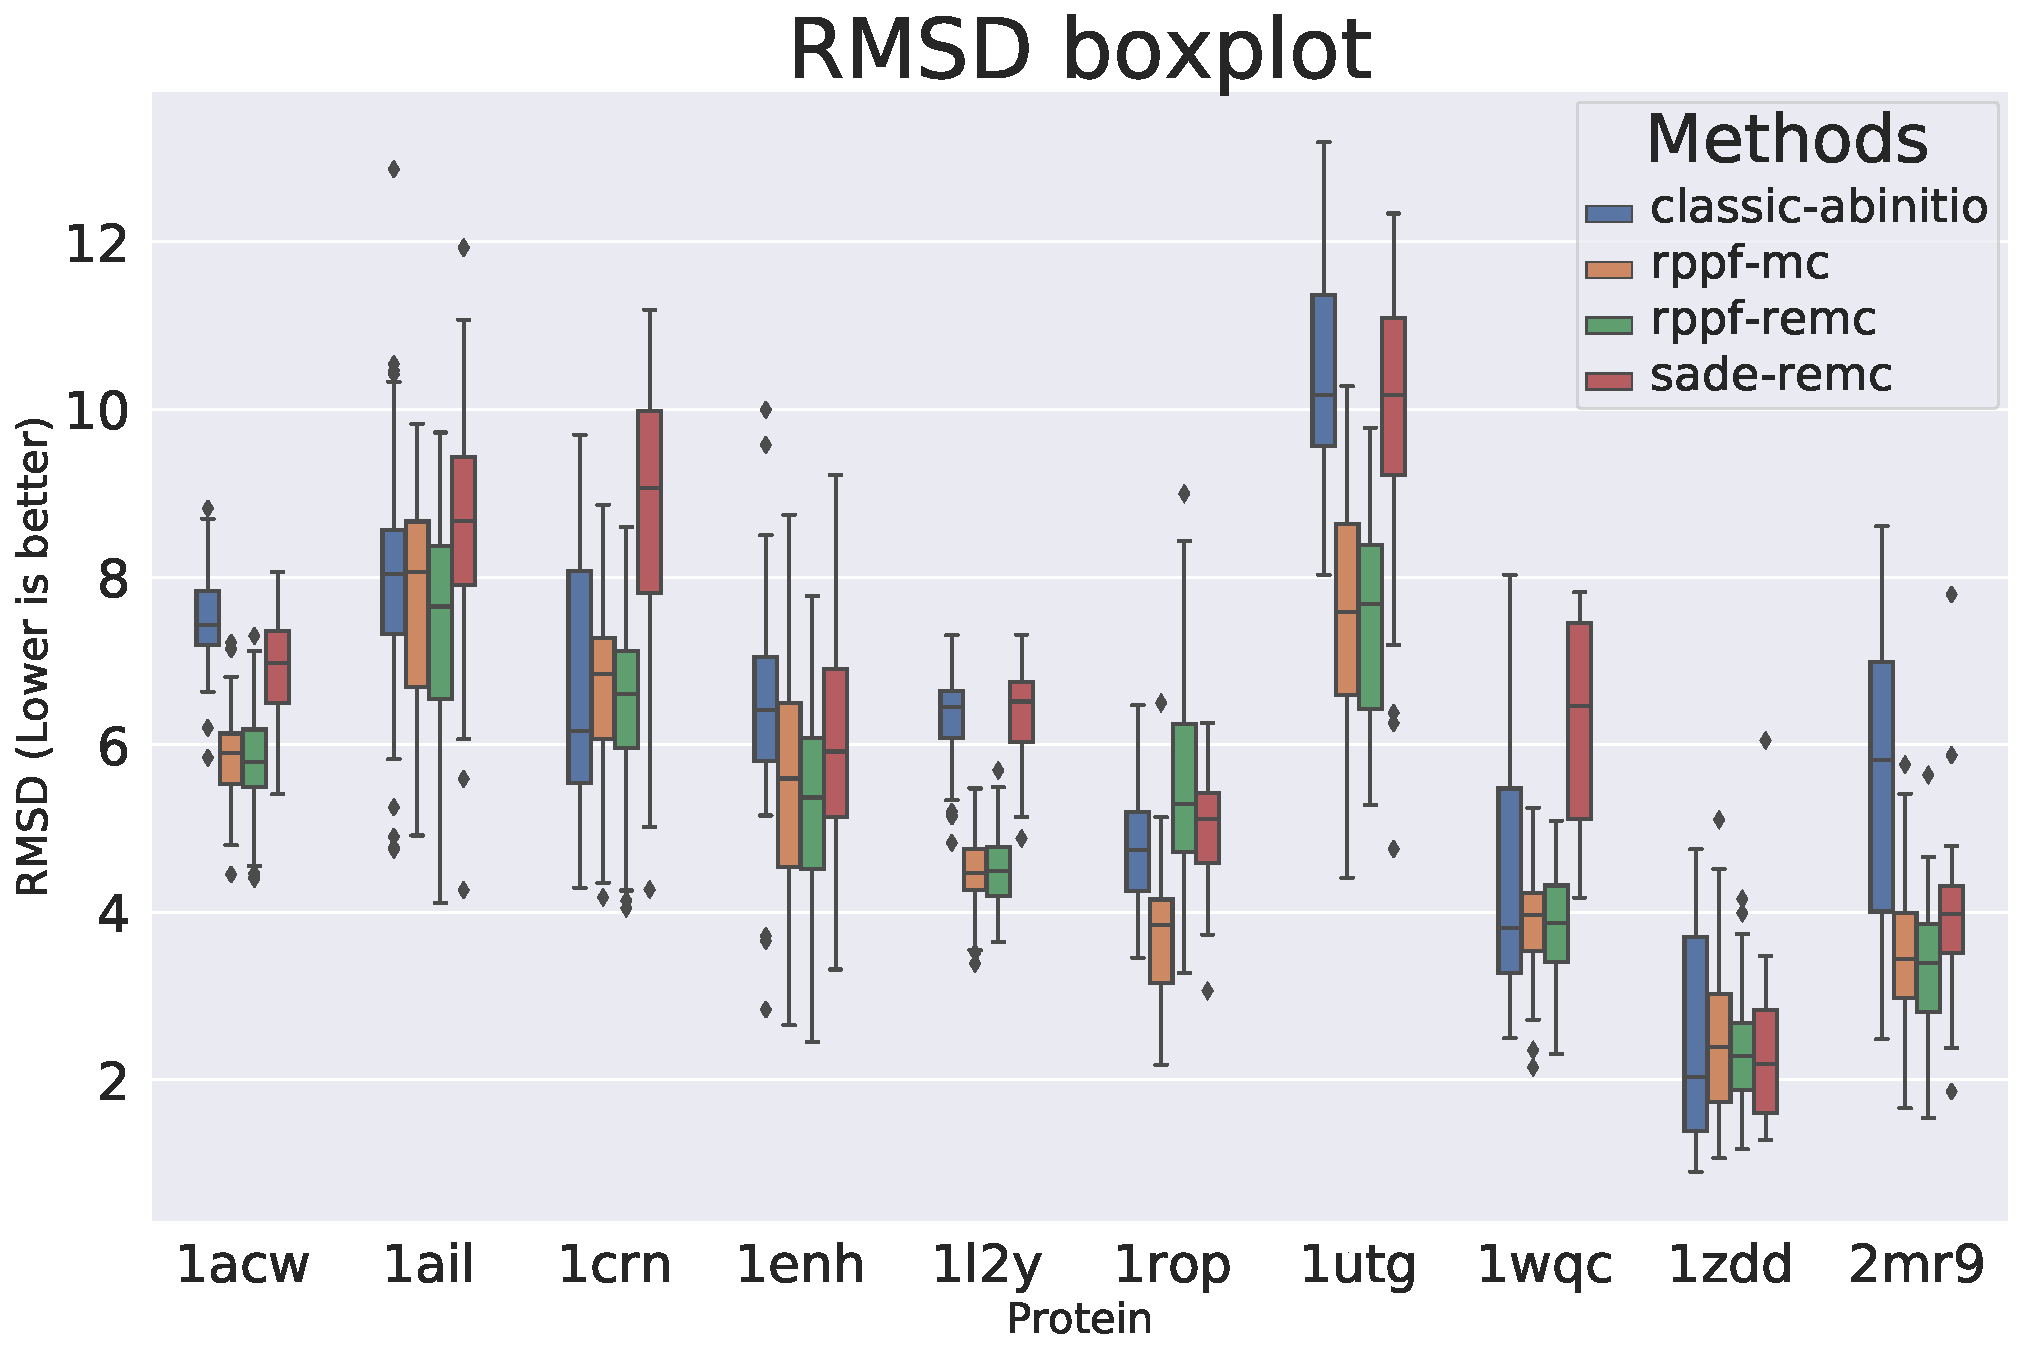
\includegraphics[width=\linewidth]{Figuras/boxplots/boxplot_best_by_rmsd_rmsd_after.pdf}
  \caption{Boxplot presenting the RMSD for the protein predictions with the
    competing methods. For the two proposed methods, the \texttt{best-by-rmsd}
    data was used}
  \label{fig:boxplot-rmsd}
\end{figure}

\begin{figure}
  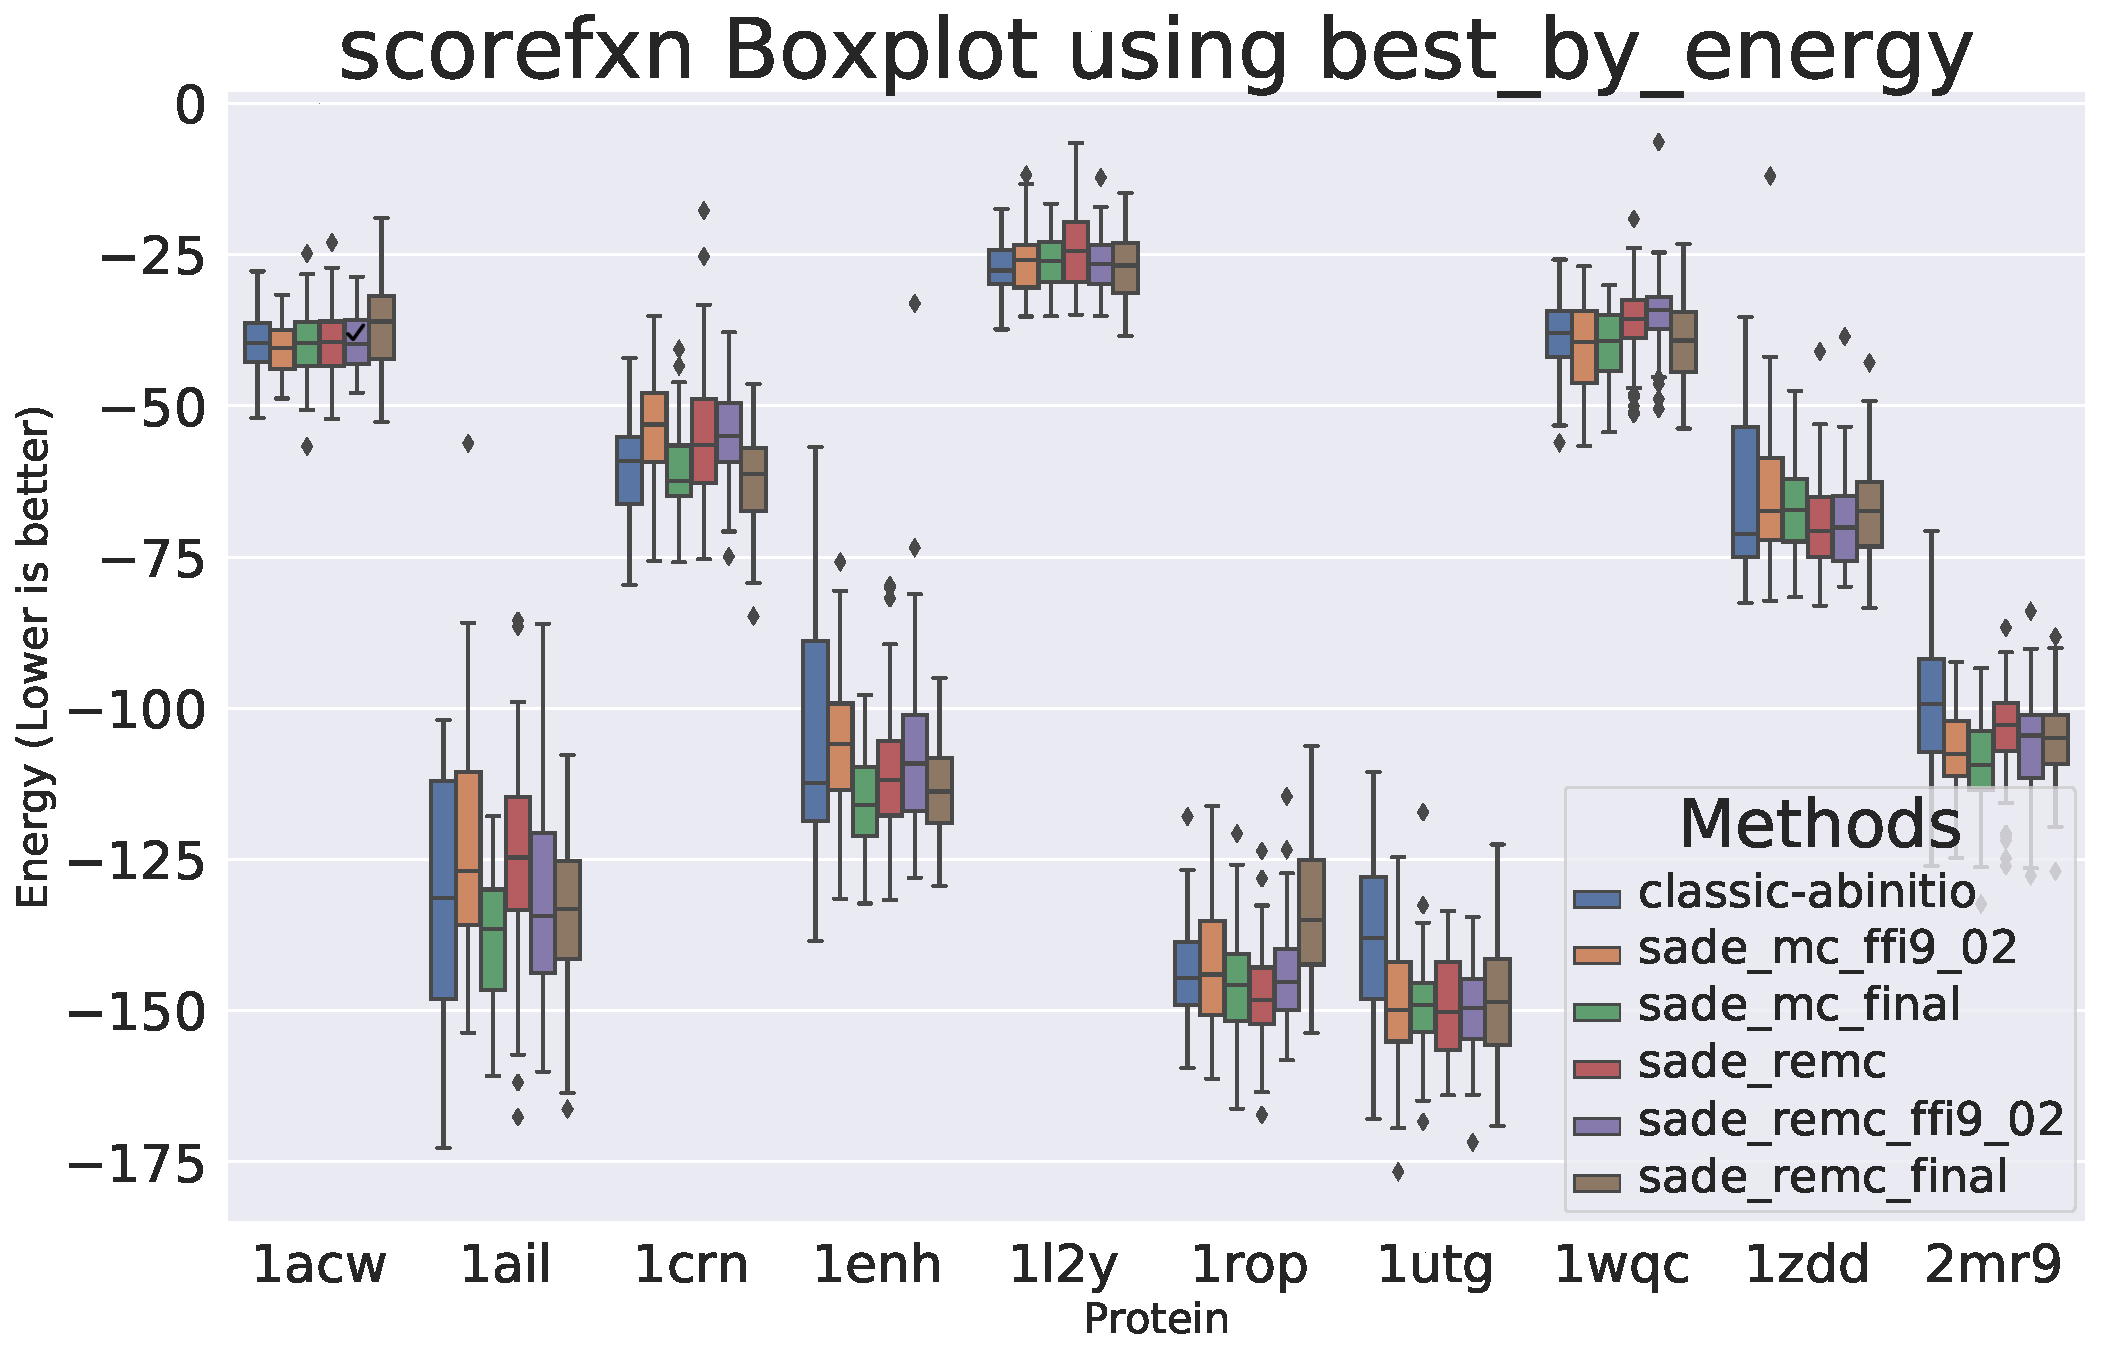
\includegraphics[width=\linewidth]{Figuras/boxplots/boxplot_best_by_energy_scorefxn.pdf}
  \caption{Boxplot presenting the \texttt{scorefxn} for the protein predictions with the
    competing methods. For the two proposed methods, the \texttt{best-by-energy}
    data was used}
  \label{fig:boxplot-energy}
\end{figure}

Figure~\ref{fig:boxplot-energy} presents data similarly to the previous figure,
however, the y axis now represents the \texttt{scorefxn} energy function. Considering
the energy results, when compared to the rmsd boxplot, the results are relativelly
more similar. Nevertheless, for some proteins there are some behaviours that are
more visible. For 1rop, sade-remc-final appears to have had a worst performance
than the other methods. Same as with the RMSD data. For 1crn, rosetta and the two
proposed methods appears to have a better result overall. For 2mr9, rosetta
appears to be lagging behind in performance. These observations are just visual
trends which helps understand the relative performance. In order to properlly
access their differences a more rigorous statistical approach is required.

% Present shapiro-wilk RESULTS
To scientifically assess the performance of the proposed methods relative to
other competing methods, proper statistical tests are required. A pre-requisite
before applying the tests which evaluate performance, is to detect the
underlying distribution of the data to be analysed. There are several ways to
acomplish this. One, is to visualy inspect a histogram or a Quartile-Quantile
plot. A more rigorous approach is to use a statistical test which can evaluate
the presence of a gaussian distribution. One such test is Shapiro-Wilk and it
will be utilized for this purpose.

For the tests an $\alpha = 0.05$ was utilized. The RMSD and \texttt{scorefxn}
of both the \texttt{best-by-rmsd} and \texttt{best-by-energy} were analysed for
all the methods. For the sake of breviety the results are exposed outside this
text, in Appendix~\ref{appendix:shapiro}.

% Present mann-whitney RESULTS

% Present Friedmann rank test RESULTS

\subsection{Pareto Front Analysis}\label{sec:pareto-front-analysis}

\subsection{Analysis Conclusions}\label{sec:analysis-conclusions}

% Analyze the overall results and conclude

\section{Convergence and Diversity Analysis}
% AVG rmsd plot

\section{Parameter Analysis and Operator Usage}
% Most used parameters over time

\section{Forced Fragment Insertion Analysis}
% What was the impact? How good/bad it was

\section{Repacking Impact}
% How much does the rmsd change before after
% If ranked by energy, does the ranking change before/after repacking

\section{Processing time}

\section{Comparison with Competing Methods}
% Big table here

\begin{sidewaystable}
  \begin{tabular}{c|l|c|c|c|c|c|c|c|c|c|c} \hline \hline
    Year & Source                            & 1ROP  & 1CRN  & 1UTG  & 1ZDD & 1ENH  & 2MR9 & 1L2Y & 1ACW  & 1AIL  & 1WQC \\ \hline \hline
%
    2019 & sade-remc-final                   & 3.28  & 4.14  & 5.28  & 1.17 & 3.26  & 1.55 & 3.65 & 4.40  & 4.79  & 2.31 \\ \hline
    2019 & sade-mc-final                     & 2.18  & 4.35  & 4.41  & 1.07 & 2.74  & 1.66 & 3.39 & 4.45  & 4.92  & 2.15 \\ \hline
%
    2019 & Rosetta                           & 3.46  & 4.30  & 8.03  & 0.91 & 2.84  & 2.48 & 4.83 & 5.85  & 4.75  & 2.50 \\ \hline
%
    2019 & {\cite{silva2019self}}            & -     & 6.08  & -     & 1.16 & 3.23  & -    & -    & -     & 4.46  & -    \\ \hline
    2019 & {\cite{narloch2019knowledge}}     & 6.02  & 4.53  & 6.38  & 2.35 & 5.56  & 2.49 & -    & 1.67  & -     & -    \\ \hline
    2018 & {\cite{song2018adoption}}         & 2.21  & 5.16  & 5.68  & 1.84 & 5.81  & -    & -    & -     & -     & -    \\ \hline
    2018 & {\cite{borguesan2018genetic}}     & -     & -     & 4.29  & -    & -     & 2.39 & -    & 2.00  & -     & -    \\ \hline
    2018 & {\cite{silva2018multistage}}      & -     & 6.96  & -     & 2.62 & 5.70  & -    & -    & -     & 8.27  & -    \\ \hline
    2017 & {\cite{de2018three}}              & 1.80  & 3.80  & 3.30  & 1.90 & 2.10  & 2.60 & 1.00 & -     & -     & 2.50 \\ \hline
    2017 & {\cite{narloch2017protein}}       & -     & 15.44 & -     & 9.42 & 19.28 & -    & -    & -     & 16.88 & -    \\ \hline
    2017 & {\cite{gao2018incorporation}}     & 3.07  & 5.34  & -     & -    & -     & -    & -    & -     & -     & -    \\ \hline
    2016 & {\cite{borguesan2016improving}}   & -     & -     & -     & -    & -     & 9.25 & -    & 11.10 & -     & 2.98 \\ \hline
    2016 & {\cite{venske2016ademo}}          & 4.48  & 6.06  & -     & -    & -     & -    & -    & -     & -     & -    \\ \hline
    2015 & {\cite{borguesan2015apl}}         & -     & 19.30 & -     & 9.50 & 20.23 & -    & -    & -     & 24.65 & -    \\ \hline
    2015 & {\cite{shehu2015review}}          & 3.37  & 4.43  & 3.60  & -    & -     & -    & -    & -     & -     & -    \\ \hline
    2015 & {\cite{rocha2015multiobjective}}  & -     & 4.98  & -     & -    & 4.23  & -    & 3.53 & -     & -     & 2.29 \\ \hline
    2013 & {\cite{olson2013off}}             & -     & -     & -     & -    & -     & -    & -    & -     & 3.90  & -    \\ \hline
    2013 & {\cite{brasil2013multiobjective}} & -     & 5.36  & -     & -    & 6.32  & -    & 2.31 & -     & -     & 2.97 \\ \hline
    2013 & {\cite{dorn2013knowledge}}        & -     & -     & -     & -    & -     & -    & 4.12 & 9.90  & -     & -    \\ \hline
    2013 & {\cite{venske2013multiobjective}} & -     & -     & -     & 2.16 & -     & -    & -    & -     & -     & -    \\ \hline
    2009 & {\cite{mansour2009scatter}}       & 17.25 & -     & 20.63 & -    & -     & -    & -    & -     & -     & -    \\ \hline
    2008 & {\cite{kehyayan2008evolutionary}} & 17.25 & -     & -     & -    & -     & -    & -    & -     & -     & -    \\ \hline
    2008 & {\cite{judy2009multi}}            & 3.48  & -     & 4.43  & 2.15 & -     & -    & -    & -     & -     & -    \\ \hline
    2006 & {\cite{cutello2005multi}}         & 3.70  & -     & 4.60  & 2.27 & -     & -    & -    & -     & -     & -    \\ \hline
  \end{tabular}
  \caption{A comparison of the RMSD from the best prediction}
  \label{tab:literature-comparison}
\end{sidewaystable}


\section{GDT-TS and TM-Score metrics}

\section{Visual Representation of the Predictions}

